\subsection{Reinforcement Learning} \label{sec: la}

Roughly speaking, reinforcement learning is an area that studies how agents can learn without the labeled example of what to do. In this case, agents learn solely from their feedback from the environment. Initially, the agent does not need to know the sequence of actions to be taken, however, the actions that optimize the fitness function should be learned along the process \cite{Sutton:1998}. Reinforcement learning serves to deal with complex systems \cite{Russell:2010}. The advantage of reinforcement learning is that this does not require any discussion of the environment model. Figure 1 shows that the supervisor only generates a reward according to feedback from the environment regardless its particular model.

\begin{figure}[!hbt]
	\begin{center}
		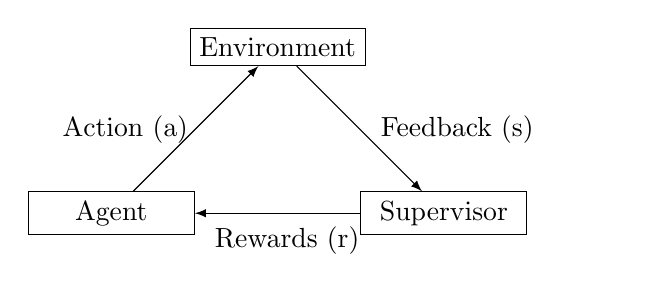
\begin{tikzpicture}[>=latex,every node/.style={rectangle,minimum width={6em},node distance=8.5em}]
		\node [draw](a) {Environment};
		\node [draw,below left of=a] (b) {Agent};
		\node [draw,below right of=a] (c) {Supervisor};
		\node [text width=3cm] at (8em, -3em) {Feedback (s)};
		\node [text width=3cm] at (-3.5em, -3em) {Action (a)};
		\node [text width=3cm] at (2em, -7em) {Rewards (r)};
		\draw [->] (b) -- (a);
		\draw [->] (a) -- (c);
		\draw [->] (c) -- (b);
		
		\end{tikzpicture}
		\caption{Diagram of reinforcement learning scheme.}
	\end{center}
	\label{diagram}
\end{figure}

According to \cite{Sutton:1998} a typical reinforcement learn model consists of:

\begin{itemize}
	\item a discrete set of environment states, $s$;
	\item a discrete set of agent actions, $a$; and
	\item a set of scalar reinforcement signals; typically {0; 1}, or the real numbers.
\end{itemize}

For this work, we use an particular approach of reinforcement learning, known as learning automata. Wu \& Liao \cite{Wu:2013} proposed learning automata in order to solve complex function optimisation problems, and named his model as Function Optimisation by Learning Automata (FOLA). These authors demonstrate that learning automata improves the optimization performance in terms of its convergence rate and accuracy, requiring less computation time in order to obtain a more accurate solutions, especially for high-dimensional functions.

In this approach, the automata updates the action probabilities according to the responses of the environment. Specifically, for this project, FALA (\emph{finite action-set learning automata}) will be used \cite{Narendra:1989}. Given the state-set $S$, FALA can be described as:

\begin{equation}
\label{eq: FALA}
\Gamma = (A,R,\tau,\overline{P}(t))
\end{equation}
where $A = \{a_0,a_1,a_2,...,a_n\}$ is the finite action-set, $R$ is the reinforcement signal-set, $\tau$ the learning scheme and $\overline{P}(t)$ is the vector or probabilities. In this case, $\overline{P}_{i}(t)$ is the probability of an action $a_i$ to be chosen at the time $t$. Notice that, I assume that $\overline{P}_{i}(t) \geq 0$ and $\sum_{i=0}^{n} \overline{P}_{i}(t) = 1$.

Thus, the vector of probabilities $\overline{P}(t)$ is updated according as following learning algorithm:

\begin{equation}
\label{eq: updateFALA}
\overline{P}_{(t+1)} = \tau(\overline{P}_{(t)},a(t),R(t))
\end{equation}
This means that the updated probability $\overline{P}_{(t+1)}$ depends on the current vector of probabilities $\overline{P}_{(t)}$, the action $i$ chosen $a_{i}(t)$ and the reward $R$ at time $t$. Basically, the process is as follow: On every moment $t$, an action $a_{i}(t)$ is taken according to the vector of probabilities $\overline{P}_{(t)}$. The output is an reaction or a change of state to $S(t+1)$. Afterward, based on the state $S(t+1)$, the quality of the result is measured and the reward is calculated according to the parameters in the set $R$. In the end, the value of $R$ is used to update the vector of probabilities $\overline{P}_{(t+1)}$ \cite{Narendra:1989}. 